\documentclass{beamer}
\usepackage[english]{layout}
\usepackage[utf8]{inputenc}
\usepackage[english]{babel}
\usepackage[T1]{fontenc}
\usepackage{amsmath, soul, color, multicol, type1cm, verbatim, latexsym, dsfont, float, listings,alltt}
\usepackage[official]{eurosym}
\usepackage{beamerthemesplit}
\usetheme{Frankfurt}
\usecolortheme{lily}
%\usefonttheme{structuresmallcapsserif}
\usefonttheme{professionalfonts}
\setbeamercovered{transparent}

%NeSI Colors <---------------------------------------------------------------------------------------
\usecolortheme[RGB={47, 68, 71}]{structure} 
\definecolor{nesidark}{HTML}{2F4447}
\definecolor{nesilight}{HTML}{CED9DF}
\definecolor{nesigrey}{gray}{0.7}
\definecolor{nesilightgrey}{gray}{0.98}
\definecolor{nesidarkgrey}{gray}{0.3}
\definecolor{nesiblue}{HTML}{2B9FC2}
\setbeamercolor{block title}{fg=black,bg=nesigrey}
\setbeamercolor{block body}{bg=nesilightgrey,fg=nesidarkgrey}
\setbeamercolor{block body alerted}{bg=white,fg=black}
\setbeamercolor{alerted text}{bg=white,fg=black}

\setbeamerfont{title}{size=\huge}
\frenchspacing
\hyphenation{NeSI}

\newcommand\BackgroundPicture[1]{%
\setbeamertemplate{background}{%
\parbox[c][\paperheight]{\paperwidth}{%
\vfill \hfill \includegraphics[height=0.9\paperheight]{#1}
\hfill \vfill
}}}

\setbeamertemplate{blocks}[default]%[shadow=false]
\useinnertheme{circles}
\setbeamertemplate{title page}[default][center,rounded=false,shadow=false]

\title{Stay Tuned}
\subtitle{How NeSI Optimises the Usage of Shared HPC Resources\\Computational Science Team @ NeSI}
\author{Jordi Blasco \\(jordi.blasco@nesi.org.nz)}
\date{}


\begin{document}

{
\setbeamertemplate{background canvas}{
\includegraphics[height=0.99\paperheight]{NeSI_img/Slide00.png}} 
\begin{frame}[plain]
\vspace{1cm}
\titlepage
\end{frame}
}


%\BackgroundPicture{NeSI_img/SlideXX.png}
\begin{frame}
\frametitle{Outline}
\begin{multicols}{2}
   \tableofcontents
 \end{multicols}
 \end{frame}


%%%%%%%%%%%%%%%%%%%%%%%%%%%%%%%%%%%%%%%%%%%%%%%%%%%%%%%%%%%%%%%%%%%%%%%%%%%%%%%%%%%%%%%%%%%%%%%
%%%%%%%%%%%%%%%%%%%%%%%%%%%%%%%%%%%%%%%%%%%%%%%%%%%%%%%%%%%%%%%%%%%%%%%%%%%%%%%%%%%%%%%%%%%%%%%



\section{About NeSI CS Team}
\subsection{Who we are?}

\frame[t]
{
  \frametitle{About NeSI CS Team}
   \begin{block}{Computational Science Team}
   \begin{center}
   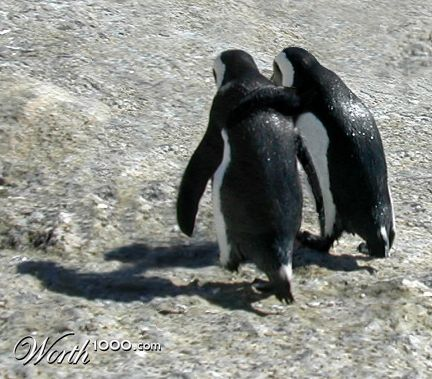
\includegraphics[width=150pt]{NeSI_img/pingu-friend.jpg}\\
   Basically, it means that we are the Researchers best friends :-)
   \end{center}
  \end{block}
}

\frame[t]
{
  \frametitle{About NeSI CS Team}
   \begin{block}{Which is the main goal of a shared HPC facility}
   \begin{itemize}%[<+-| alert@+>]
	\item Run few jobs really fast? - no matter what their efficiency are.
	\item Run the maximum number of jobs? - in favour of short and small jobs. 
	\item NeSI provides a wise combination by optimising the usage of computational resources.
   \end{itemize}
  \end{block}
}

\section{Identify the Bottlenecks}
\subsection{Identify the Most Popular Apps}
\frame[t]
{
  \frametitle{Identify the Most Popular Apps}
    %  \begin{block}{Top application list}
    \begin{figure}
         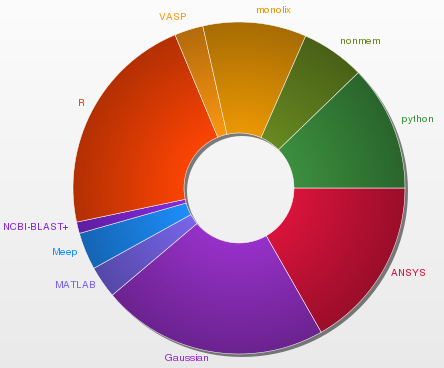
\includegraphics[width=0.6\textwidth]{NeSI_img/apps_cputime2.png}
         \caption{Most popular applications in Pan cluster. We are using \href{https://github.com/a2o/snoopy}{snoopy} to track the applications run in the cluster. This allow us to get a list of the most popular apps.}
    \end{figure}   
  %\end{block}
}

   \frame[t]
{
  \frametitle{Tuning}
 \begin{block}{Tuning the most popular applications provides a major impact in}
   \begin{itemize}%[<+-| alert@+>]
	\item the walltime of the users of this code.
	\item the global cluster efficiency.
	\item the availability of the computational resources.
	\item the waiting time.
   \end{itemize}   
   \begin{center}
   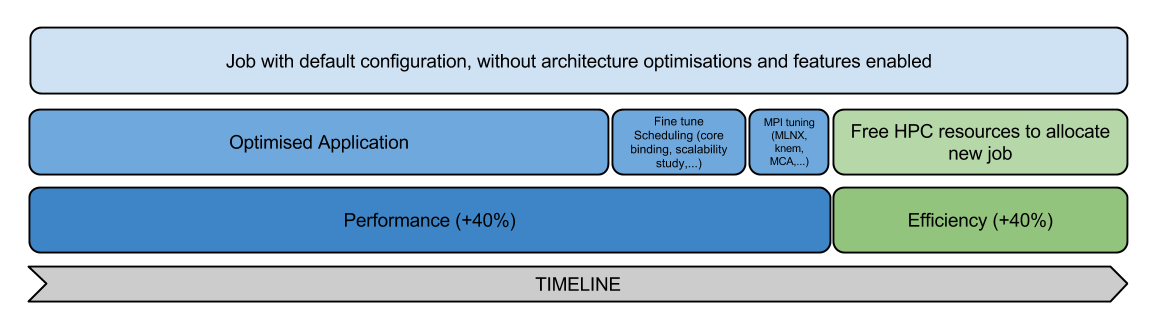
\includegraphics[width=\textwidth]{NeSI_img/Performance_improvements.png}
   \end{center}
  \end{block}
}


\section{Tuning}
\frame[t]
{
  \frametitle{Tuning}
  \begin{block}{There are several ways to tune an HPC Application}
   \begin{itemize}%[<+-| alert@+>]
	\item Most obvious : tune the algorithm.
	\item Choose the right Libraries + Compilers + MPI "Flavour".
	\item Choose the right Options and Environment.
	\item Work in the work-flow.
	\item Explore the scalability (how well it scales).
	\item Check if benchmark results are good enough.
   \end{itemize}
  \end{block}
}

\subsection{Profile and Debug}
\frame[t]
{
  \frametitle{Profile and Debug}
 \begin{block}{Available software}
   \begin{itemize}%[<+-| alert@+>]
	\item Intel Vtune Amplifier \& Intel Trace Analyzer 
	\item DDT
	\item Score-P
	\item HPC Toolkit
	\item Scalasca
	\item Cube
	\item PAPI
	\item TAU
	\item Parallel Profile Visualization (ParaProf)
	\item Native Slurm profiling tools
   \end{itemize}
  \end{block}
}

\subsection{Increase the performance}
\frame[t]
{
  \frametitle{Increase the performance}
  \begin{block}{PhyML Case Study - Dr. Stéphane Guindon (UoA)}
  \textbf{PhyML} is a software that estimates maximum likelihood phylogenies from alignments of nucleotide or amino acid sequences. The main strength of PhyML lies in the large number of substitution models coupled to various options to search the space of phylogenetic tree topologies, going from very fast and efficient methods to slower but generally more accurate approaches.
  \end{block}
  \begin{block}{Using the right tools}
In this case, the right compilers and optimization options for an specific architecture increased the performance up to x6.
  \end{block}
}

\frame[t]
{
  \frametitle{Increase the performance}
      \begin{block}{PhyML Case Study : Speed Up}
\begin{center}
 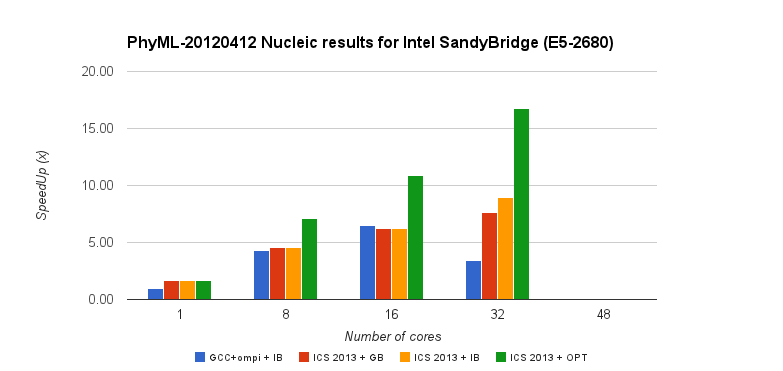
\includegraphics[width=\textwidth]{NeSI_img/speedup-phyml.png}
\end{center}
  \end{block}
}

\frame[t]
{
  \frametitle{Increase the performance}
      \begin{block}{PhyML Case Study : Performance}
\begin{center}
 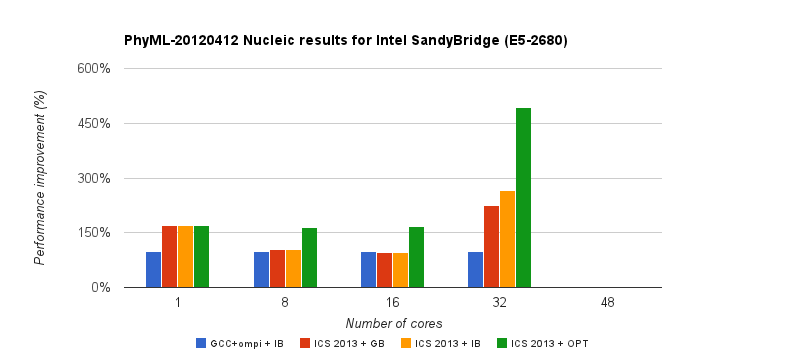
\includegraphics[width=\textwidth]{NeSI_img/performance-phyml.png}
\end{center}
  \end{block}
}

\subsection{Discover the scalability limits}
\frame[t]
{
  \frametitle{Discover the scalability limits}
     \begin{block}{How well the code scales?}
 % \begin{center}
 \begin{itemize}
 \item There are theoretical limits but the reality can be really surprising!
 \item The scalability/quality of a code is measured in terms of efficiency (USL).
 \item The benchmarks can help to discover the real scalability limits.
 \item With this information you can get even faster results and save computational resources for other jobs.
 \end{itemize}
  %\end{center}
  \end{block}
}


\frame[t]
{
  \frametitle{Discover the scalability limits}
      \begin{block}{Migrate-n Case Study - Dr. Sarah Knight (UoA)}
Migrate estimates effective population sizes and past migration rates between n population assuming a migration matrix model with asymmetric migration rates and different subpopulation sizes.
  \end{block}
}


\frame[t]
{
  \frametitle{Discover the scalability limits}
      \begin{block}{Migrate-n Case Study}
\begin{center}
 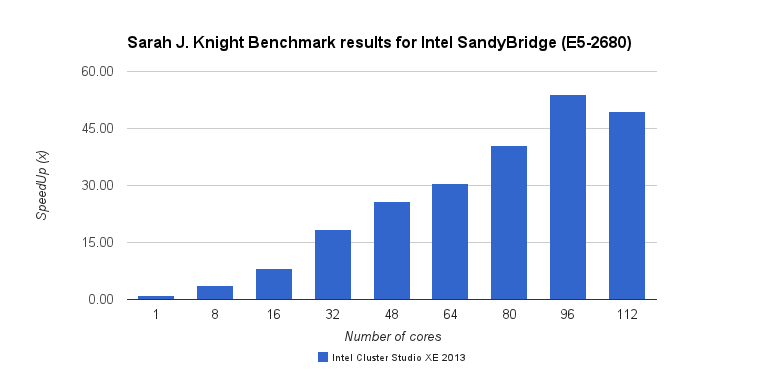
\includegraphics[width=\textwidth]{NeSI_img/scalability-migrate-n.png}
\end{center}
  \end{block}
}

\frame[t]
{
  \frametitle{Discover the scalability limits}
  \begin{block}{Is the scalability as good as you expect?}
  \begin{center}
  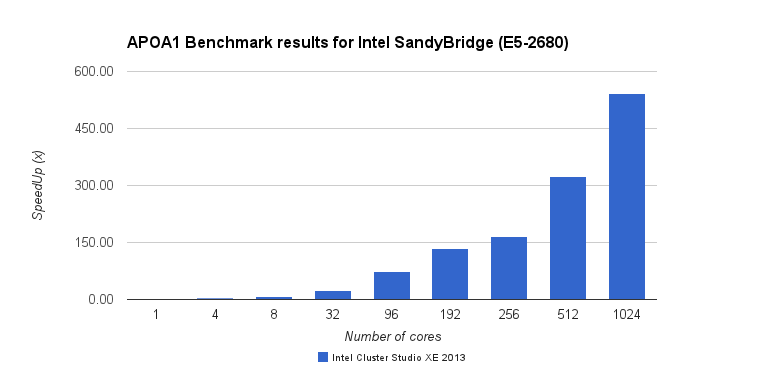
\includegraphics[width=\textwidth]{NeSI_img/speedup-namd.png}\\
  \end{center}
  \end{block}
}

\subsection{Improve the efficiency}
\frame[t]
{
  \frametitle{Improve the efficiency}
      \begin{block}{The workflow can save several HPC resources}
 \begin{itemize}
 \item Thanks to the nature of some codes, the problem can be transformed into a embarrassing parallel problem.
 \item In some cases it's possible to split large input file into several small files, allowing to run several copies of the same code using  completely independent input files.
 \item In scenarios like these you can achieve a linear scalability.
 \item Several problems related with genomics have this approach.
 \end{itemize}
  \end{block}
}


\frame[t]
{
  \frametitle{Improve the efficiency}
      \begin{block}{NCBI-BLAST+ Case Study}
BLAST (Basic Local Alignment Search Tool) command line applications developed at the National Center for Biotechnology Information (NCBI).
  \end{block}
  \begin{block}{Benchmark provided by Dr. Daniel White (Landcare Research)}
 It describes the dataset as a pathogen discovery dataset using de novo metagenomics.
  \end{block}
}

\frame[t]
{
  \frametitle{Improve the efficiency}
      \begin{block}{NCBI-BLAST+ Case Study : Speed Up}
\begin{center}
 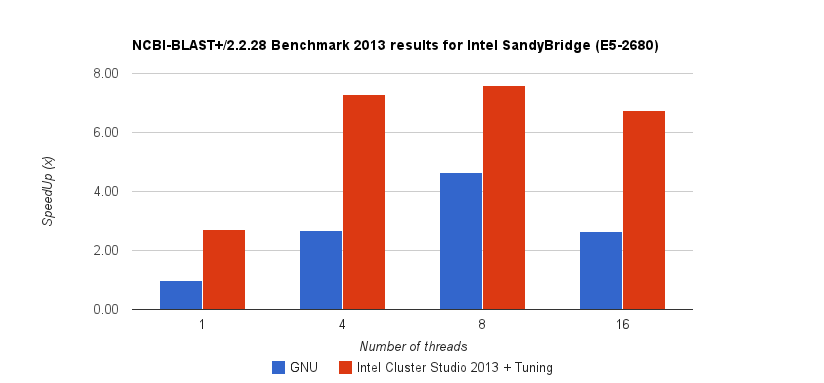
\includegraphics[width=\textwidth]{NeSI_img/speedup-blast.png}
\end{center}
  \end{block}
}


\frame[t]
{
  \frametitle{Improve the efficiency}
      \begin{block}{NCBI-BLAST+ Case Study : Efficiency}
\begin{center}
 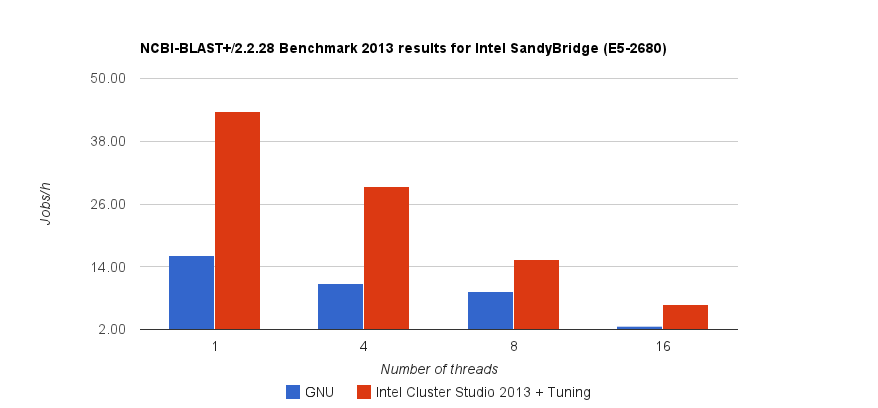
\includegraphics[width=\textwidth]{NeSI_img/jobsh-blast.png}
\end{center}
  \end{block}
}

\frame[t]
{
  \frametitle{Improve the efficiency}
      \begin{block}{NCBI-BLAST+ Case Study : Speed Up compared with original code}
\begin{center}
\begin{tabular}{|c|c|c|c|c|c|}
\hline 
threads & split & tuned binaries & SHM & Speed Up & Efficiency \\ 
\hline 
1 & 1000 & 2.71 & • & • & • \\ 
\hline 
4 & 1000 & 7.27 & • & • & • \\ 
\hline 
8 & 1000 & 7.61 & • & • & • \\ 
\hline 
16 & 1000 & 6.74 & • & • & • \\ 
\hline 
\end{tabular} 
\end{center}
  \end{block}
}

\section{Back to the future}
\subsection{Moore's Law}
\frame[t]
{
  \frametitle{Back to the future}
      \begin{block}{Moore's Law}
\begin{center}
  \vspace{-0.3cm}
  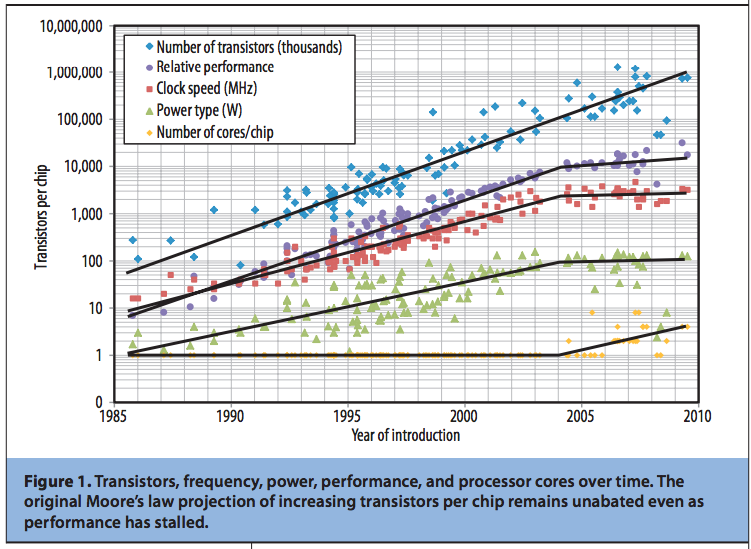
\includegraphics[width=0.80\textwidth]{NeSI_img/Moores-law.png}
\end{center}
  \end{block}
}



\subsection{Sequencing cost}
\frame[t]
{
  \frametitle{Back to the future}
      \begin{block}{Sequencing Cost per Genome}
\begin{center}
 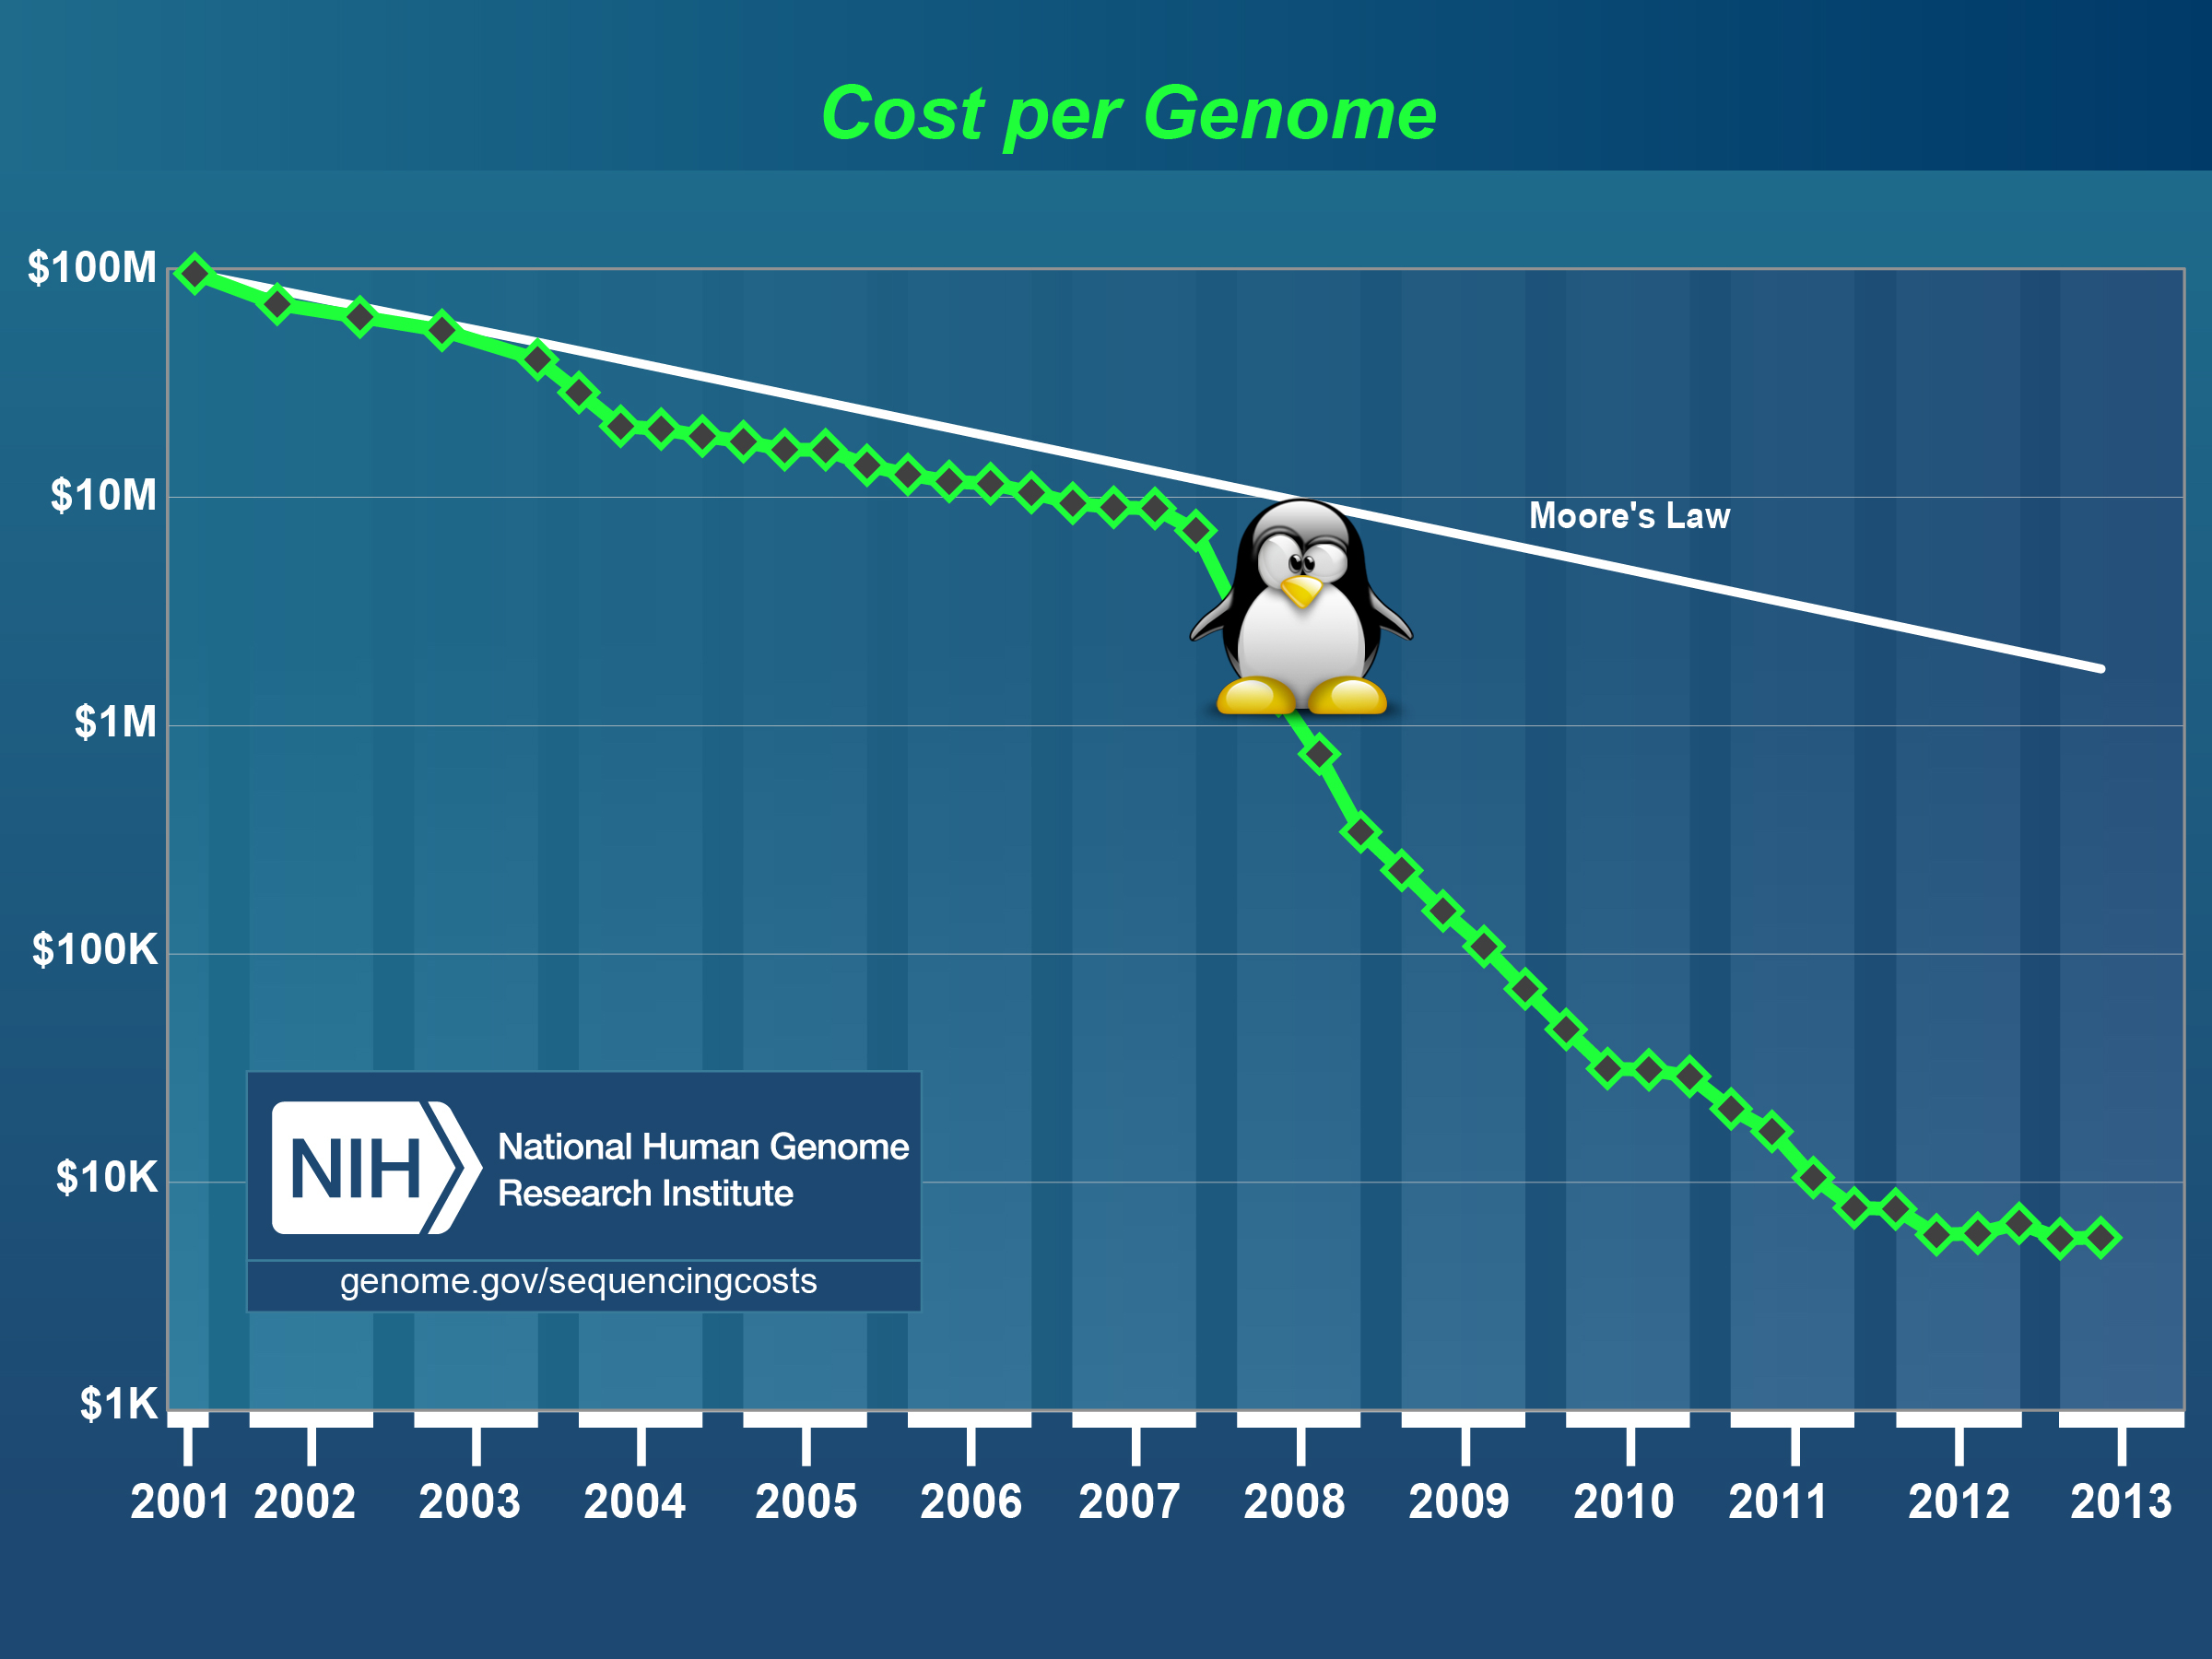
\includegraphics[width=0.75\textwidth]{NeSI_img/cost_per_genome_apr01.jpg}
\end{center}
  \end{block}
}

\frame[t]
{
  \frametitle{Back to the future}
%      \begin{block}{Sequencing Cost per Genome}
\begin{center}
 
\includegraphics[width=0.98\textwidth]{NeSI_img/bttf-logo.png}
\end{center}
%  \end{block}
}

\frame[t]
{
  \frametitle{Back to the future}
      \begin{block}{Sequencing Cost per Genome}
\begin{center}
 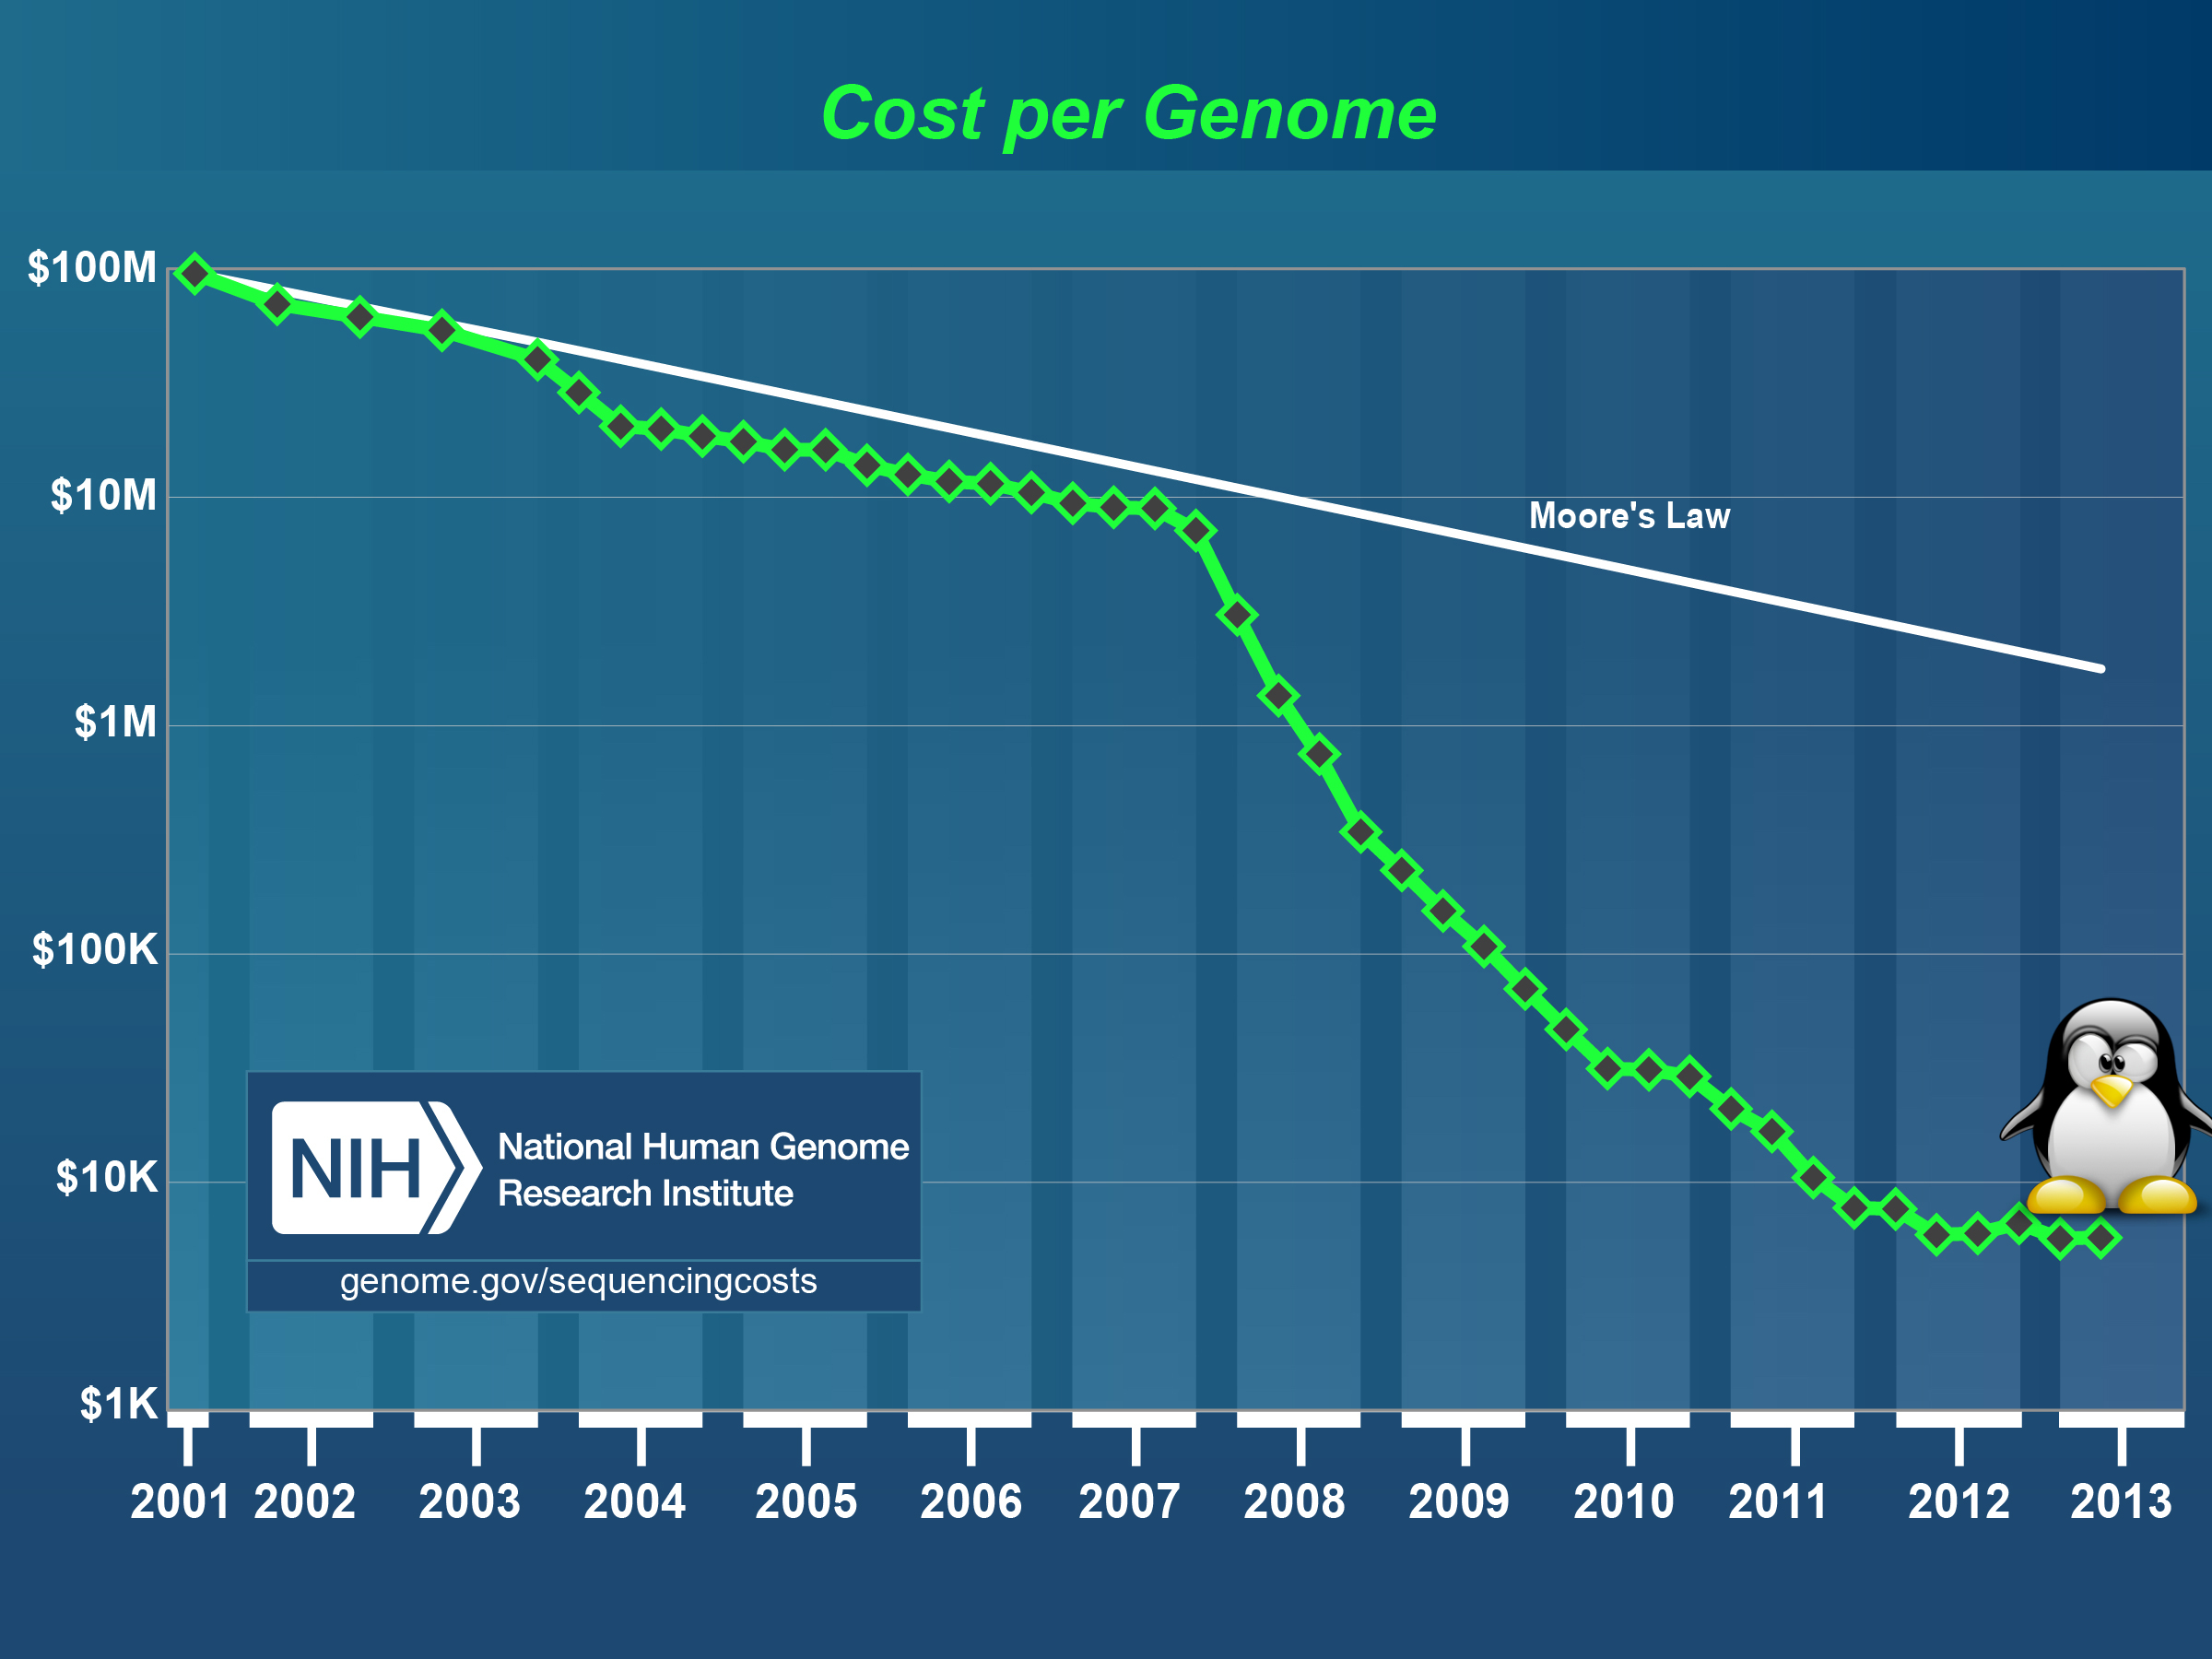
\includegraphics[width=0.75\textwidth]{NeSI_img/cost_per_genome_apr02.jpg}
\end{center}
  \end{block}
}

\frame[t]
{
  \frametitle{Back to the future}
      \begin{block}{Are you still living in the 80's?}
\begin{center}
 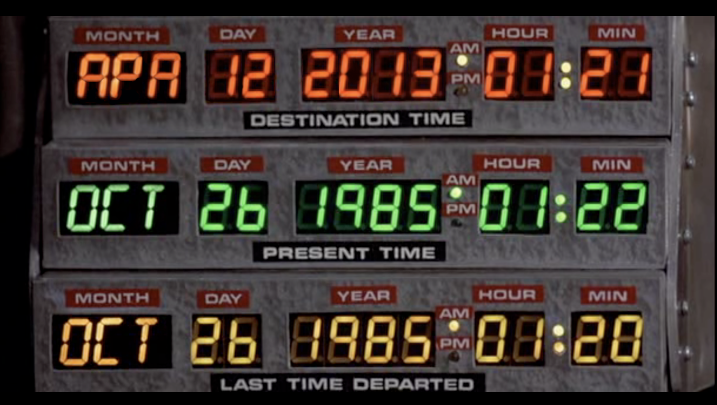
\includegraphics[width=0.8\textwidth]{NeSI_img/back2thefuture-clock.png}
\end{center}
  \end{block}
}


\frame[t]
{
%  \frametitle{}
\begin{center}
 
\includegraphics[width=\textwidth]{NeSI_img/Stay-Tuned.jpg}
\end{center}
}

{
\setbeamertemplate{background canvas}{
\includegraphics[height=0.99\paperheight]{NeSI_img/Slide00.png}} 
\begin{frame}[plain]
\begin{center}
{\Huge Questions \& Answers}
\end{center}
\end{frame}
}


\end{document}